\chapter{Objetivos, planificación y presupuesto}
\section{Objetivos}\label{objetivos}
\subsection{Obtención y relación de patrones}
Sacar mediante expresiones regulares datos de interés de correos electrónicos y relacionarlos entre sí. Esto permitirá a los expertos del sector contar con una herramienta para poder realizar análisis de mayor profundidad al poder relacionar datos comunes entre los distintos correos de la base de datos. 

Un ejemplo sencillo de esto puede ser el análisis de un correo electrónico nuevo, pero con una url ya conocida y presente en otros correos electrónicos. 

Un ejemplo más complejo podría ser, el análisis de un mensaje con una url nueva, pero con un dominio de cuya IP sí se tienen registros, lo que puede dar lugar a una nueva línea de investigación sobre si dicho dominio pertenece (O no) a un cibercriminal, aunque no se tengan registros previos ni del dominio ni de la url en cuestión. 

Se debe extraer al menos los siguientes tipos de datos:
\begin{itemize}
    \item Direcciones IP
    \item Dominios
    \item Enlaces
    \item Direcciones de correo electrónico
\end{itemize}

Aunque el servicio se debe pensar para que en un futuro se puedan extraer más tipos de datos como carteras de criptomonedas o números de teléfono.

\subsection{Evaluar de manera relativa la maliciosidad}
Se deben detectar ciertas técnicas comúnmente usadas por los ciberdelincuentes para atacar a sus víctimas y así asignar un valor de maliciosidad tanto a los datos extraídos como a los mensajes en sí. 

Algunas de estar técnicas podrían ser: 
\begin{itemize}
    \item Mostrar un enlace distinto al que se redirige.
    \item Usar una gran cantidad de subdominios de subdominios
    \item Mostrar un correo electrónico distinto del real
\end{itemize}

\subsection{Ofrecer un servicio de análisis público}
La segunda parte del proyecto será ofrecer a todos los usuarios la posibilidad de analizar sus mensajes mediante una web donde podrán o bien copiar y pegar el mensaje, o bien subir un archivo eml para un análisis más completo. 

La página devolverá varias listas con todos los tipos datos extraídos del análisis, así como enlaces a cada uno de ellos donde se muestre un informe más detallado.

Esto permitirá que a un usuario que le llegue un correo y no sepa si es o no malicioso, pueda analizarlo en la página y obtener más información sobre este.

\subsection{Cumplir de manera efectiva con la ley de protección de datos}
Es de vital importancia diseñar el servicio pensando en las leyes de protección de datos, especialmente en la europea por ser la más estricta hasta el momento. 

Los usuarios deben poder eliminar, tanto los mensajes, como los datos obtenidos de ellos si así lo desean de manera automática y sin necesidad de que nadie intervenga en el proceso. 

Aunque esta característica no se implemente en este proyecto, sí que se debe pensar el sistema para que se pueda implementar en el futuro de manera sencilla y modificando la mínima cantidad de código posible. 

\subsection{Monetización}
Como parte complementaria se intentará pensar cómo obtener ingresos económicos del desarrollo. Estos ingresos nunca deben impedir que usuarios particulares puedan usar el servicio, aunque sí pueden impedir acceder a todas las funcionalidades de este. 

\subsection{Integración con terceros}
Aunque esto está un poco al margen del TFG, sería muy interesante la integración directa desde la página con otros servicios como el de Virus Total o la de Have I been pwned.

Esto permitiría por un lado facilitar a los usuarios menos técnicos un análisis rápido desde la propia página y por otro puede dar información relevante a los expertos.

\subsection{Crear un servicio funcional}
Al final del proyecto se debe crear un servicio que dé un soporte real y online, no se debe limitar a tener un servicio local únicamente de prueba. Por lo que durante el apartado del diseño se deben elegir tecnologías factibles para su posterior despliegue en internet y por tanto no limitadas a un entorno de local pruebas.

\section{Planificación}
Para la planificación se ha usado un diagrama de Gantt (Ver figura \ref{fig:Gantt}).
En él se puede ver como se le ha dado prioridad a la búsqueda de información, en concreto a la base de datos, pues se considera que es una parte crucial del proyecto. 

Por otro lado, en la implementeación se ha dado prácticamente el mismo tiempo al diseño y creación de la base de datos, como a la parte de programación del análisis. 

También se ha dejado bastante tiempo a la creación de las expresiones regulares para la búsqueda de patrones, ya que hay varias expresiones que crear y no se tiene mucho conocimiento sobre este tema. 

La parte más rápida sería la creación de la web, ya que es donde se tiene más experiencia e incluso posría reutilizarse trabajo prévio. 

En total y si se cumplen los plazos, el desarrollo del proyecto llevaría 120 días.

Como metodología de desarrollo de software se utilizarán prototípos evolutivos. Esto va a permitir centrarse al principio en las característica principales y sobre esas ir añadiendo nuevas funcionalidades. Por ejemplo hacer el desarrollo únicamnete para un patrón y en la siguente evolución añadir otro. 

\begin{figure}[htb]
    \centering
    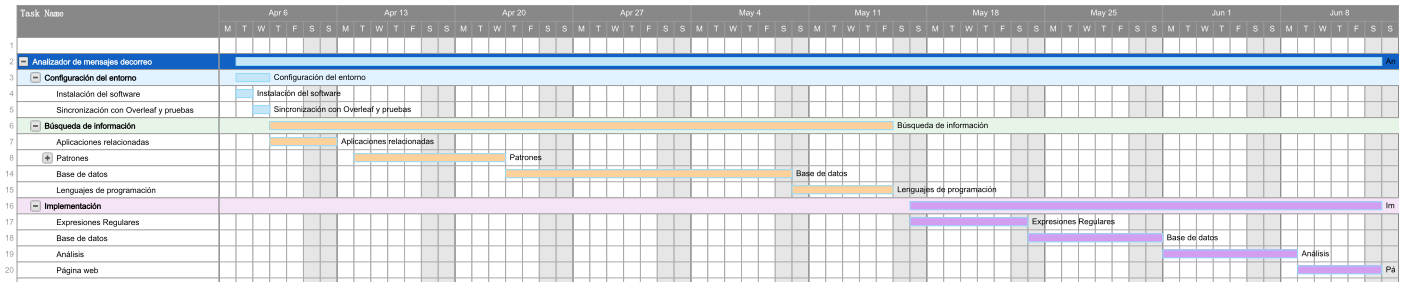
\includegraphics[width=\textwidth]{imagenes/Diagrama_Gann.png}
\caption{Diagrama de Gantt}
\label{fig:Gantt}
\end{figure}

\section{Presupuesto}

En la parte del presupuesto (Ver figura \ref{fig:Presupuesto}) se ha tenido en cuenta:
\begin{itemize}
    \item El coste del equipo utilizado (700€) y una amortización en 2 años.
    \item La mano de obra, que serían 120 días como se ha visto en el apartado de planificación, trabajando 8h al día ya que se va a trabajar a tiempo completo y a 22€/h ya que va a trabajar como autónomo.
    \item El hosting donde se va a desplegar el proyecto que tiene un coste de 120€ al año.
\end{itemize}

Sumando todos los costes, el precio final del proyecto serían unos \textbf{21.355€}.

\begin{figure}[htb]
    \centering
    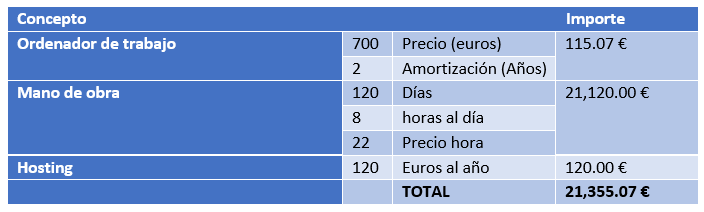
\includegraphics[width=0.8\textwidth]{imagenes/Presupuesto.png}
\caption{Presupuesto del proyecto.}
\label{fig:Presupuesto}
\end{figure}